\documentclass[10pt]{article}

\input{packages.tex}
\input{commands.tex}
\input{header.tex}

\usepackage{titlesec}
\usepackage{csquotes}
\usepackage{subcaption}
\usepackage[style=numeric,backend=biber]{biblatex}

\titleformat*{\section}{\large\bfseries}
\titleformat*{\subsection}{\bfseries}

\begin{document}
\header{}
\vskip 12pt

\begin{center}
\Large\textbf{Single Run Report}
\end{center}

The run started at \VAR{starttime} and the root machine was \VAR{hostname}. The simulation used \VAR{world_size} processes to simulate \VAR{nb_particles} particles in a total of \VAR{nb_cells} cells, i.e. \VAR{nb_cells_per_layer} cells per process. The runtime for the simulation was: \VAR{runtime}. Figure \ref{fig:loading} displays the loading of the processes over the runtime.\\

The simulation used a total of \VAR{nb_total_send} MPI\_Send \& MPI\_Recv calls which excludes calls after the simulation end to aggregate statistics data.


\begin{figure}[h]
    \centering
    \includegraphics[width=\textwidth]{fig01.png}
    \caption{Load for all processes. Process 0 is shown at the top. The sum of all times (stack height) should equal the statistics\_cycle\_time, i.e. \VAR{statistics_cycle_time} sec. If processes are idle it is a "good" sign because at least no CPU Power is wasted while no computation is available. Also see Figure \ref{fig:loadingb}}
    \label{fig:loading}
\end{figure}


\FloatBarrier
\begin{table}[hbt]
\centering
\begin{tabular}{l | l}
$x_{min}$ & \VAR{x_min} \\
$x_{max}$ & \VAR{x_max} \\
$x_{ini}$ & \VAR{x_ini} \\
particle\_min\_weight & \VAR{particle_min_weight} \\
nb\_particles & \VAR{nb_particles} \\
max\_used\_buffer\_size & \VAR{max_used_buffer} \\
max\_possible\_buffer\_size & \VAR{buffer_size} \\
cycle\_time & \VAR{cycle_time} \\
cycle\_nb\_steps & \VAR{cycle_nb_steps} \\
statistics\_cycle\_time & \VAR{statistics_cycle_time}\\
world\_size & \VAR{world_size}
\end{tabular}
\caption{The configuration values used for this run.}
\label{tab:config}
\end{table}

\begin{figure}[htb]
    \centering
    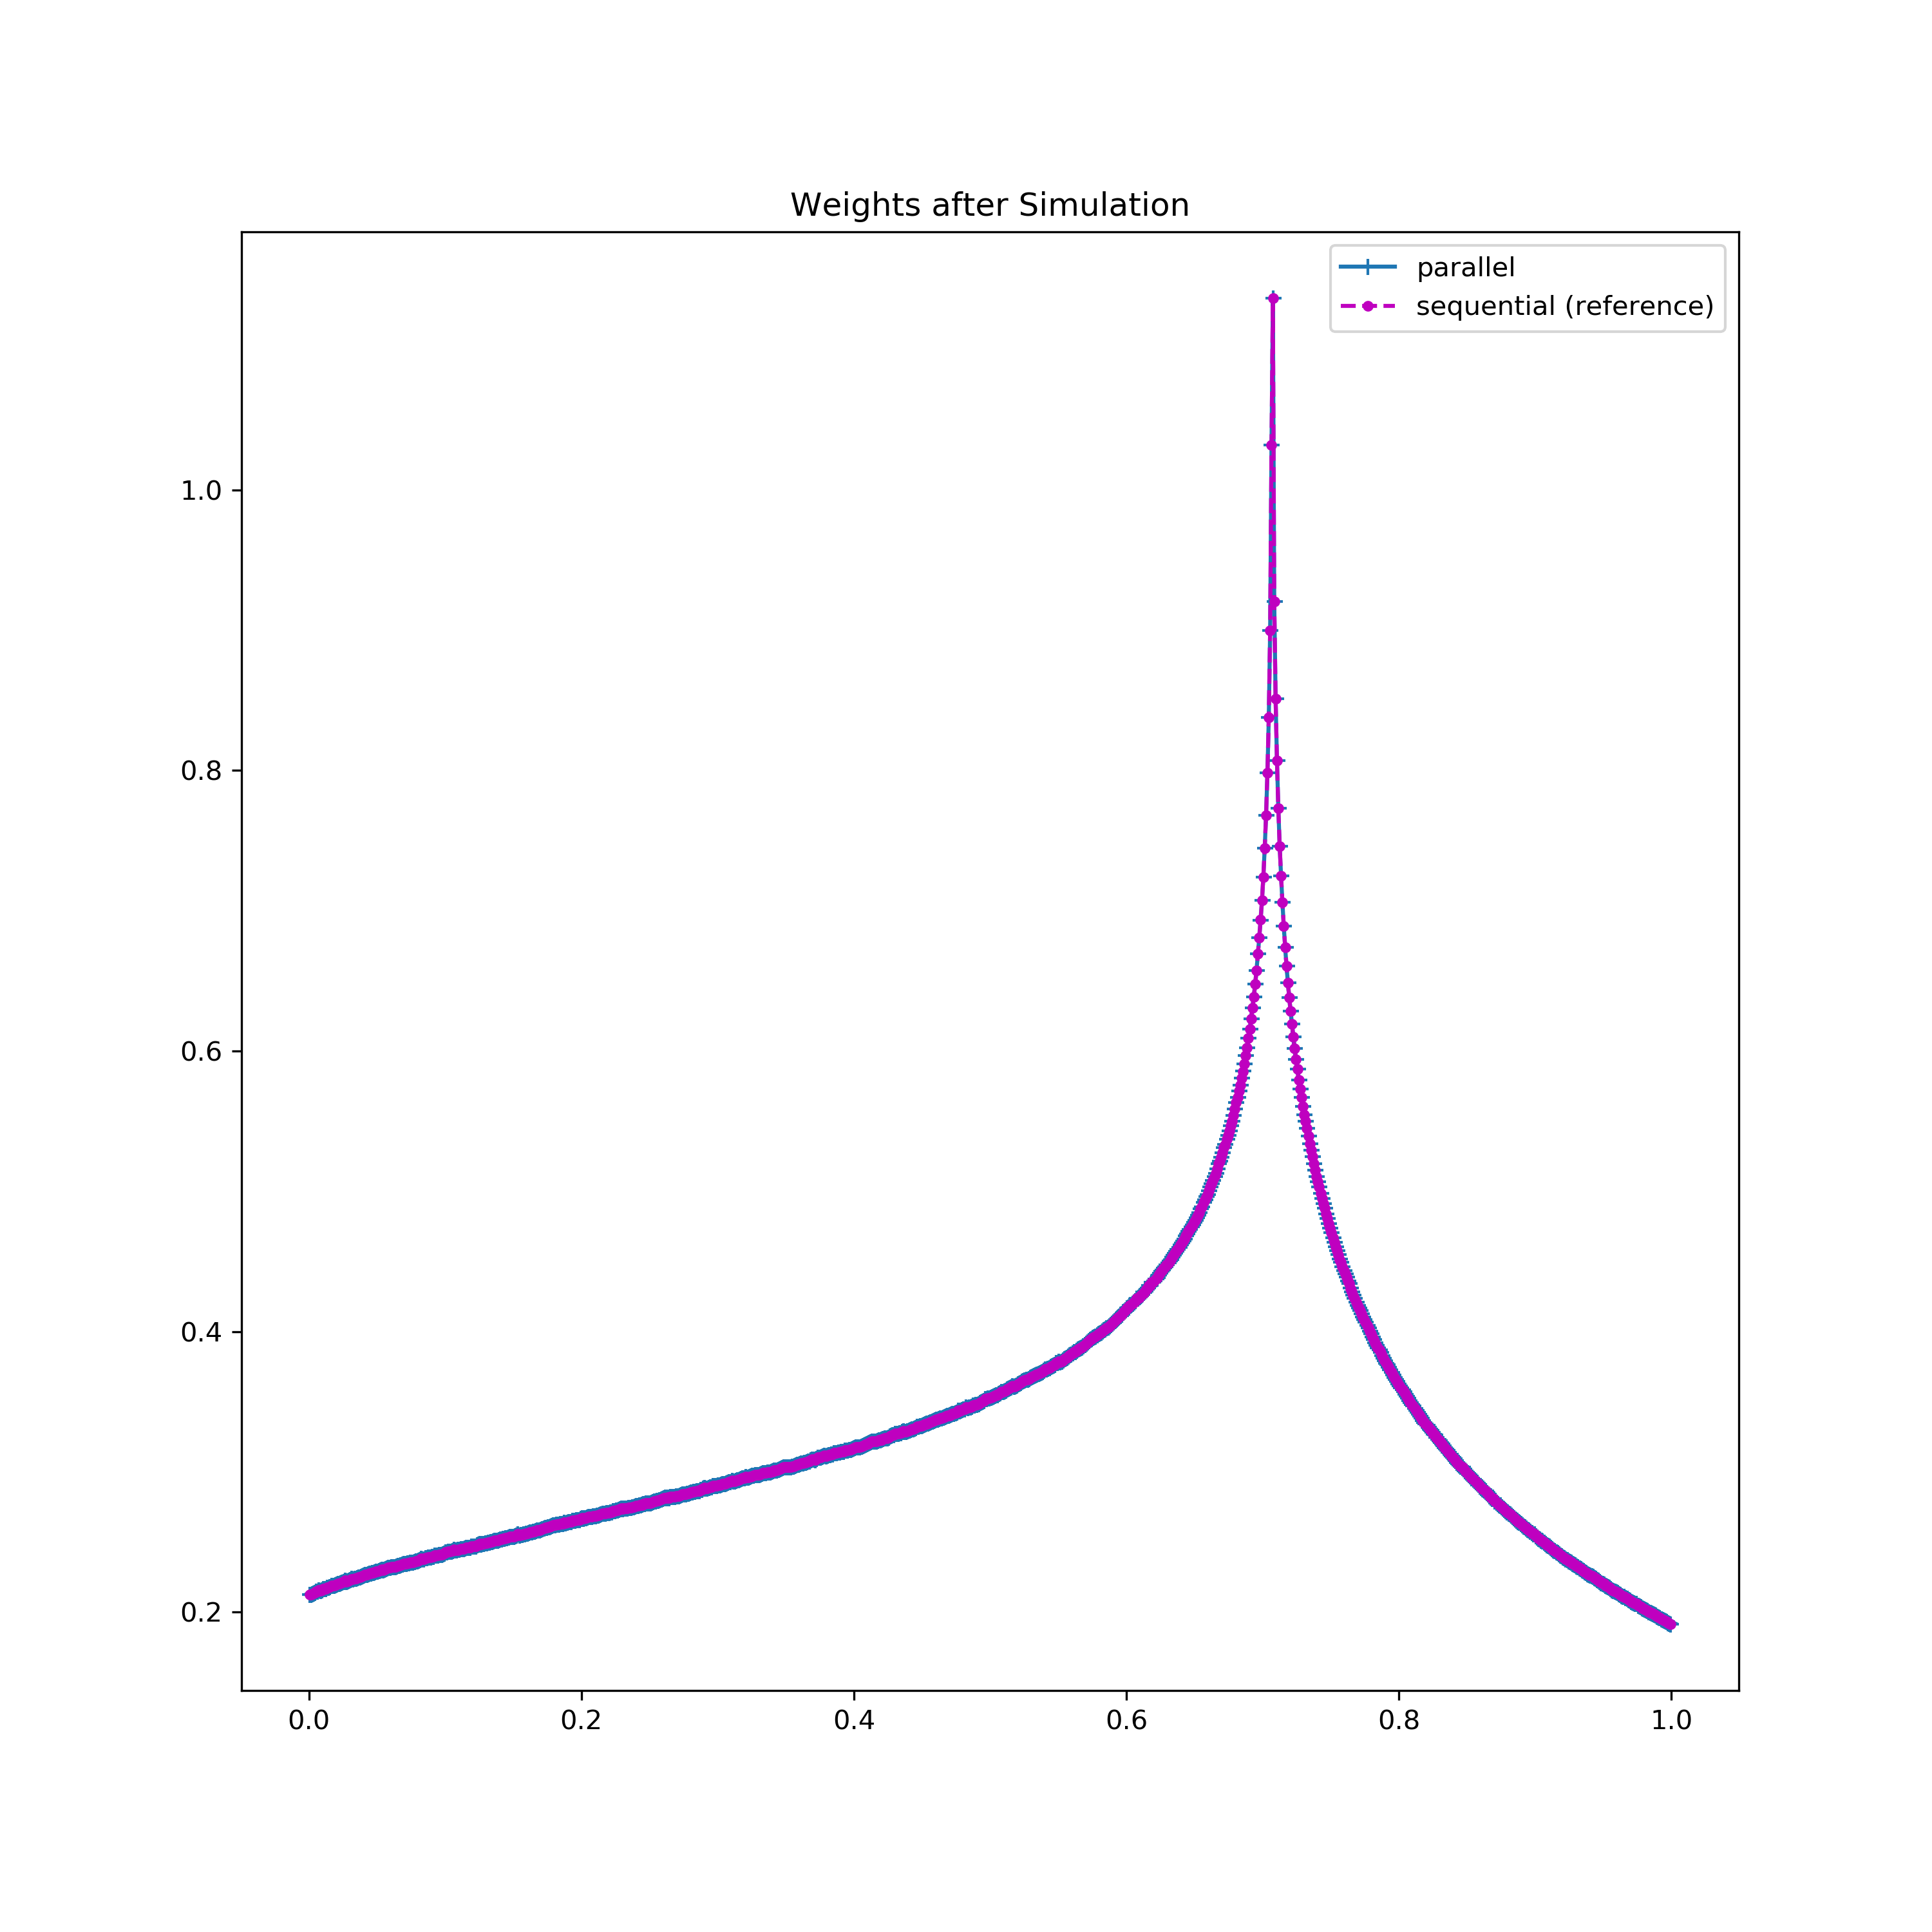
\includegraphics[width=\textwidth]{fig_weights.png}
    \caption{Weights to compare parallel and sequential code (should be identical).}
    \label{fig:weights}
\end{figure}

\begin{figure}[h]
    \centering
    \includegraphics[width=\textwidth]{fig01b.png}
    \caption{First second of loading.}
    \label{fig:loadingb}
\end{figure}

\end{document}